\documentclass[fleqn, a4paper, 10pt, oneside]{amsart}
\usepackage{exsheets}
\usepackage{amsmath, amssymb, amsthm} %standard AMS packages
\usepackage{marginnote} %marginnotes
\usepackage{gensymb} %miscellaneous symbols
\usepackage{commath} %differential symbols
\usepackage{xcolor} %colours
\usepackage{cancel} %cancelling terms
\usepackage[free-standing-units, space-before-unit]{siunitx} %formatting units
\usepackage{tikz, pgfplots} %diagrams
	\usetikzlibrary{calc, hobby, patterns, intersections, decorations.markings}
\usepackage{graphicx} %inserting graphics
\usepackage{hyperref} %hyperlinks
\usepackage{datetime} %date and time
\usepackage{enumerate,enumitem} %numbered lists
\usepackage{float} %inserting floats
\usepackage{circuitikz}[american voltages, american currents] %circuit diagrams
\usepackage{booktabs}
\usepackage{csvsimple}
\usepackage{todonotes}

\newcommand\numberthis{\addtocounter{equation}{1}\tag{\theequation}} %adds numbers to specific equations in non-numbered list of equations

\theoremstyle{definition}
\newtheorem{example}{Example}
\newtheorem{definition}{Definition}

\theoremstyle{theorem}
\newtheorem{theorem}{Theorem}

\makeatletter
\@addtoreset{section}{part} %resets section numbers in new part
\makeatother

\SetupExSheets{solution/print = true}

%opening
\title
[
	Electronic Devices : Assignment 5
]
{
	Electronic Devices\\
	Assignment 5
}
\author
{
	Aakash Jog\\
	ID : 989323563
}
\date{\formatdate{14}{4}{2016}}

\begin{document}

\maketitle
%\setlength{\mathindent}{0pt}

\begin{question}
	Shown below are the electron and hole current densities in an ideal PN junction in forward bias.
	\begin{figure}[H]
		\centering
		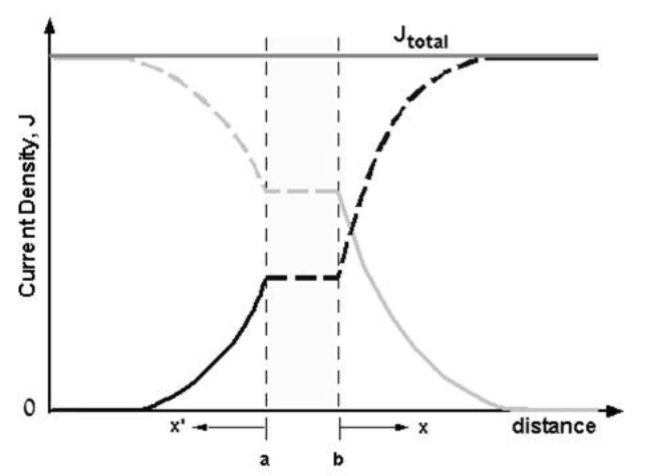
\includegraphics[width = 0.5\textwidth]{fig1.png}
	\end{figure}
	\begin{enumerate}
		\item
			Given that the current density $J$ is directed towards the right, which side is N-type and which side is P-type?
		\item
			If we assume, for this question only, that the diffusion coefficients and minority carrier lifetimes of electrons and holes are equal, what can we say about the doping concentrations?
		\item
			As shown, the current densities in the depletion region are constant due to which of the following?
			\begin{enumerate}
				\item Depletion approximation
				\item Negligence of recombination in the depletion region
				\item Strong electric fields in the depletion region
				\item Boltzmann approximation
			\end{enumerate}
		\item
			If at the edge of the depletion region, the electron current density is equal to the hole density, which of the following conditions must be true?
			\begin{enumerate}
				\item $N_A D_p = N_D D_n$
				\item $\frac{D_p}{N_A L_n} = \frac{D_n}{N_D L_p}$
				\item $N_A L_p = N_D L_n$
				\item $\frac{D_n}{N_A L_n} = \frac{D_p}{N_D L_p}$
				\item $N_A = N_D$
			\end{enumerate}
	\end{enumerate}
\end{question}

\begin{solution}
	\begin{enumerate}[leftmargin=*]
		\item
			As the junction is in forward bias, and the current density is directed towards the right, the junction is a PN junction.
		\item
			In the depletion region, hole current is greater than the electron current.
			Therefore, the concentration of holes is greater than that the concentration of electrons.
			Therefore, $N_A > N_D$.
		\item
			As the current densities are constant in the depletion region, the concentration of electrons and holes across the depletion region must be constant.
			Therefore, there is no generation and recombination in the depletion region.
		\item
			\begin{align*}
				J_n &= J_p\\
				\therefore \frac{D_p}{L_p} {p_N}_0 &= \frac{D_n}{L_n} {n_P}_0\\
				\therefore \frac{D_p}{L_p} \frac{{n_i}^2}{N_D} &= \frac{D_n}{L_n} \frac{{n_i}^2}{N_A}\\
				\therefore \frac{D_p}{L_p} N_A &= \frac{D_n}{L_n} N_D
			\end{align*}
	\end{enumerate}
\end{solution}

\begin{question}
	Consider a silicon PN step junction diode at $300 \kelvin$, with
	\begin{align*}
		N_A &= 5 \times 10^{15} \si{\per\centi\metre\cubed}\\
		N_D &= 10^{15} \si{\per\centi\metre\cubed}\\
		A &= 10^{-4} \si{\centi\metre\squared}\\
		\tau_n &= 0.4 \si{\micro\second}\\
		\tau_p &= 0.1 \si{\micro\second}\\
		\mu_n &= 1350 \si{\centi\metre\squared\per\volt\per\second}\\
		\mu_p &= 480 \si{\centi\metre\squared\per\volt\per\second}
	\end{align*}
	\begin{enumerate}
		\item Calculate the reverse hole current, i.e. the hole current when $V_a < 0$.
		\item Calculate the reverse electron current, i.e. the electron current when $V_a < 0$.
		\item Calculate the hole concentration at $x_n$ for $V_a = 0.5 V_{\text{BI}}$.
		\item Calculate the electron current at $x = x_n + \frac{L_p}{2}$ for $V_a = 0.5 V_{\text{BI}}$.
	\end{enumerate}
\end{question}

\begin{solution}
	\begin{enumerate}[leftmargin=*]
		\item
			\begin{align*}
				J_p(x) &= q \left( \frac{D_p}{L_p} {p_N}_0 \right) \left( e^{\frac{q V_a}{k T}} - 1 \right) e^{-\frac{x}{L_p}}\\
				&= q \left( \frac{D_p}{\sqrt{D_p \tau_p}} \frac{{n_i}^2}{N_D} \right) \left( e^{\frac{q V_a}{k T}} - 1 \right) e^{-\frac{x}{\sqrt{D_p \tau_p}}}\\
				&= q \left( \frac{\sqrt{D_p}}{\sqrt{\tau_p}} \frac{{n_i}^2}{N_D} \right) \left( e^{\frac{q V_a}{k T}} - 1 \right) e^{-\frac{x}{D_p \tau_p}}\\
				&= q \left( \frac{\sqrt{\frac{\mu_p k T}{q}}}{\sqrt{\tau_p}} \frac{{n_i}^2}{N_D} \right) \left( e^{\frac{q V_a}{k T}} - 1 \right) e^{-\frac{q x}{\mu_p k T \tau_p}}\\
				&= \left( 1.6 \times 10^{-19} \right) \left( \frac{\sqrt{(480) (0.026)}}{\sqrt{\left( 10^{-7} \right)}} \frac{10^{20}}{10^{15}} \right) (-1) e^{-\frac{x}{(480) (0.026) \left( 10^{-7} \right)}}\\
				&= -\left( 1.6 \times 10^{-19} \right) \left( \frac{12.48}{3.16 \times 10^{-4}} 10^5 \right) e^{-\frac{x}{1.248 \times 10^{-6}}}\\
				&= -\left( 1.6 \times 10^{-19} \right) \left( 3.95 \times 10^9 \right) e^{-\left( 8 \times 10^5 \right) x}\\
				&= -6.32 e^{-\left( 8 \times 10^5 \right) x} 10^{-10}
			\end{align*}
			Therefore,
			\begin{align*}
				I_p(x) &= J_p(x) A\\
				&= \left( -6.32 e^{\left( 8 \times 10^5 \right) x} 10^{-10} \right) \left( 10^{-4} \right)\\
				&= -6.32 e^{\left( 8 \times 10^5 \right) x} 10^{-14}
			\end{align*}
		\item
			\begin{align*}
				J_n(x) &= q \left( \frac{D_n}{L_n} {n_P}_0 \right) \left( e^{\frac{q V_a}{k T}} - 1 \right) e^{-\frac{x}{L_n}}\\
				&= q \left( \frac{D_n}{\sqrt{D_n \tau_n}} \frac{{n_i}^2}{N_A} \right) \left( e^{\frac{q V_a}{k T}} - 1 \right) e^{-\frac{x}{\sqrt{D_n \tau_n}}}\\
				&= q \left( \frac{\sqrt{D_n}}{\sqrt{\tau_n}} \frac{{n_i}^2}{N_A} \right) \left( e^{\frac{q V_a}{k T}} - 1 \right) e^{-\frac{x}{D_n \tau_n}}\\
				&= q \left( \frac{\sqrt{\frac{\mu_n k T}{q}}}{\sqrt{\tau_n}} \frac{{n_i}^2}{N_A} \right) \left( e^{\frac{q V_a}{k T}} - 1 \right) e^{-\frac{q x}{\mu_n k T \tau_n}}\\
			\end{align*}
		\item
			\begin{align*}
				p(x) &= {p_N}_0 \left( e^{\frac{q V_a}{k T}} - 1 \right) e^{-\frac{x}{L_p}}\\
				&= \frac{{n_i}^2}{N_D} \left( e^{\frac{q V_{\text{BI}}}{k T}} - 1 \right) e^{-\frac{x}{L_p}}\\
				&= \frac{10^{20}}{10^{15}} \left( e^{\frac{V_{\text{BI}}}{0.026}} - 1 \right) e^{-\left( 8 \times 10^5 \right) x}\\
				&= 10^5 \left( e^{\frac{V_{\text{BI}}}{0.026}} - 1 \right) e^{-\left( 8 \times 10^5 \right) x}
			\end{align*}
			Therefore,
			\begin{align*}
				p(x_n) &= 10^5 \left( e^{\frac{V_{\text{BI}}}{0.026}} - 1 \right) e^{-8 x_n \times 10^5}
			\end{align*}
		\item
			\begin{align*}
				J_n(x) &= q \left( \frac{D_n}{L_n} {n_P}_0 \right) \left( e^{\frac{q V_a}{k T}} - 1 \right) e^{-\frac{x}{L_n}}\\
				&= q \left( \frac{D_n}{\sqrt{D_n \tau_n}} \frac{{n_i}^2}{N_A} \right) \left( e^{\frac{q V_a}{k T}} - 1 \right) e^{-\frac{x}{\sqrt{D_n \tau_n}}}\\
				&= q \left( \frac{\sqrt{D_n}}{\sqrt{\tau_n}} \frac{{n_i}^2}{N_A} \right) \left( e^{\frac{q V_a}{k T}} - 1 \right) e^{-\frac{x}{D_n \tau_n}}\\
				&= q \left( \frac{\sqrt{\frac{\mu_n k T}{q}}}{\sqrt{\tau_n}} \frac{{n_i}^2}{N_A} \right) \left( e^{\frac{q V_a}{k T}} - 1 \right) e^{-\frac{q x}{\mu_n k T \tau_n}}\\
			\end{align*}
			Therefore,
			\begin{align*}
				J_n\left( x_n + \frac{L_p}{2} \right) &= q \left( \frac{\sqrt{\frac{\mu_n k T}{q}}}{\sqrt{\tau_n}} \frac{{n_i}^2}{N_A} \right) \left( e^{0.013 V_{\text{BI}}} - 1 \right) e^{-\frac{x_n + \frac{L_p}{2}}{0.026 \mu_n \tau_n}}\\
			\end{align*}
	\end{enumerate}
\end{solution}

\end{document}
